\documentclass{article}
\usepackage{lmodern}
\usepackage[T1]{fontenc}
\usepackage{shapepar}
\usepackage{microtype}
\usepackage{lipsum}
\usepackage{pgfplots}
\pgfplotsset{compat=1.9}
\usepackage{tikz}
\usetikzlibrary{calc,fit,intersections,folding}
\usepackage{pstricks-add}
\usetikzlibrary{arrows.meta,angles,arrows,quotes,backgrounds}


\newcommand{\clrone}{blue}
\newcommand{\clrtwo}{red}

\begin{document}
\thispagestyle{empty}
    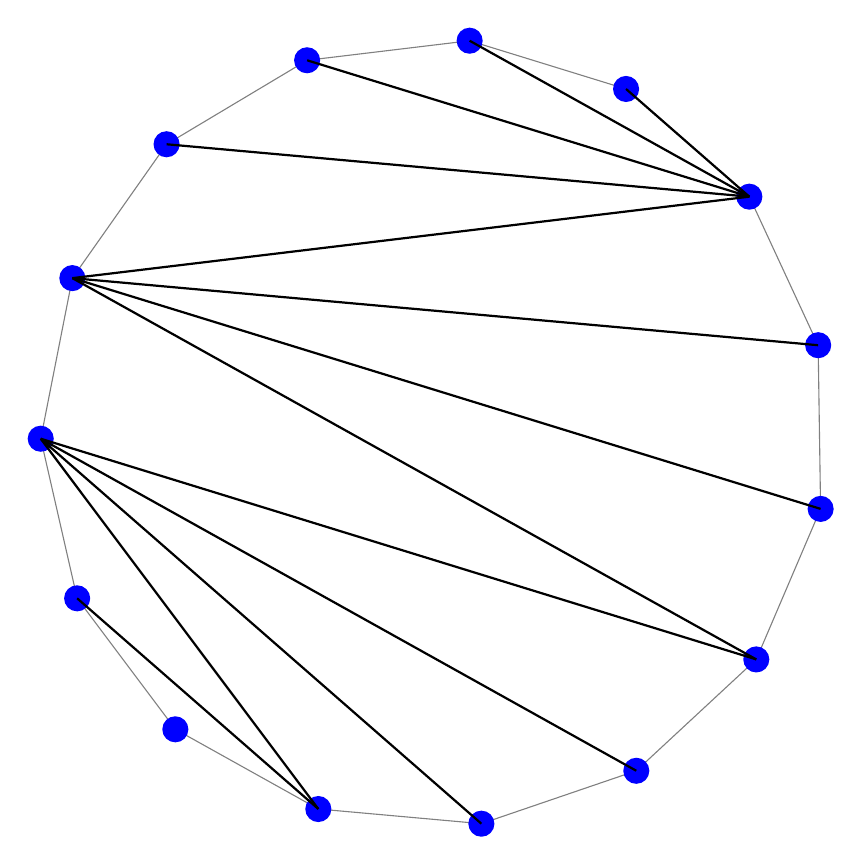
\begin{tikzpicture}[rotate = 12.86]
    %blue points
        \foreach \i in {1,...,15} {
            \node[fill, \clrone, circle] (\i) at (360*\i/15:5) {};
        }
        \begin{scope}[on background layer]
            \foreach \i in {1,...,14} {
                \pgfmathparse{int(\i+1)}
                \draw[gray] (\i.center) -- (\pgfmathresult.center);
            }
            \draw[gray] (15.center) -- (1.center);
        \end{scope}

        \foreach \x/\y in 
        {1/2, 1/3, 1/4, 1/5, 1/6, 6/15, 6/14, 6/13, 13/7, 7/12, 7/11, 7/10, 10/8}
        {
            \draw[thick] (\x.center) -- (\y.center);
        }
    \end{tikzpicture}
\end{document}